\documentclass[tikz,border=8pt]{standalone}
\usetikzlibrary{arrows.meta,positioning}

\definecolor{ink}{HTML}{17383D}
\definecolor{muted}{HTML}{6B8185}
\definecolor{green}{HTML}{3EBC83}
\definecolor{teal}{HTML}{35AFC0}
\definecolor{violet}{HTML}{6A5AE0}
\definecolor{amber}{HTML}{E7AE43}

\begin{document}
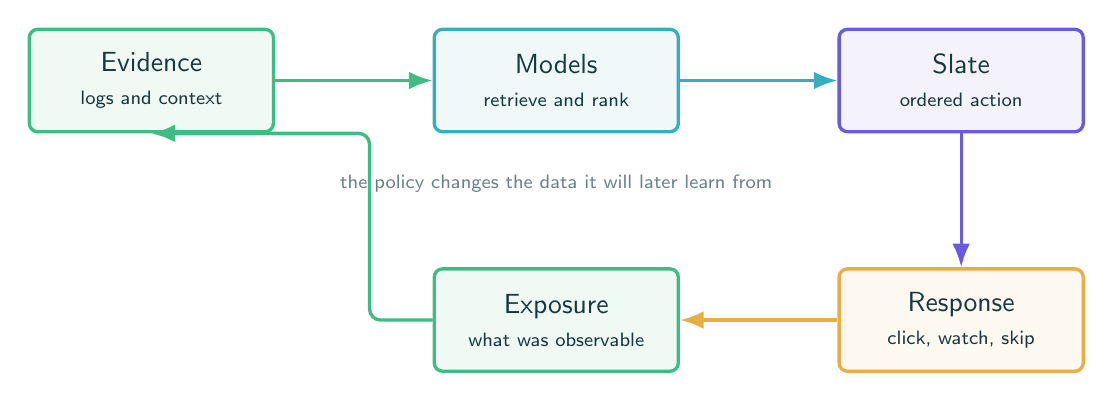
\begin{tikzpicture}[
  font=\sffamily,
  node distance=17mm and 20mm,
  stage/.style={draw=#1, fill=#1!8, text=ink, very thick, rounded corners=3pt,
    minimum width=31mm, minimum height=13mm, align=center},
  flow/.style={-{Latex[length=3mm]}, very thick, rounded corners=4pt}
]
  \node[stage=green] (evidence) {Evidence\\{\scriptsize logs and context}};
  \node[stage=teal, right=of evidence] (models) {Models\\{\scriptsize retrieve and rank}};
  \node[stage=violet, right=of models] (slate) {Slate\\{\scriptsize ordered action}};
  \node[stage=amber, below=of slate] (response) {Response\\{\scriptsize click, watch, skip}};
  \node[stage=green, left=of response] (exposure) {Exposure\\{\scriptsize what was observable}};

  \draw[flow, green] (evidence) -- (models);
  \draw[flow, teal] (models) -- (slate);
  \draw[flow, violet] (slate) -- (response);
  \draw[flow, amber] (response) -- (exposure);
  \draw[flow, green] (exposure.west) -- ++(-8mm,0) |- (evidence.south);

  \node[text=muted, font=\sffamily\scriptsize, below=4mm of models]
    {the policy changes the data it will later learn from};
\end{tikzpicture}
\end{document}
